\chapter{Design}

The focus of the application is to simplify the setup process for the therapist, ensuring that he does not require programming experience or knowledge about the underlying system, while still providing all tools needed for the patients to play a game using gesture input.\\

The developed application can roughly be split up into three major parts. Firstly, the graphical user interface (GUI) allows the therapist to interact with the application, providing him with feedback and feedforward on inputting exercises for the patients. Secondly, gesture recognition is done as part of machine learning using support vector machines (SVM). Thirdly, all other back-end software connects the first two parts and provides a structure in which all data is managed and stored.


\section{Description of the application}

The application uses Microsoft's Kinect 2.0 camera as an input device. The principle is that games can be played by first recording gestures and then performing them. In order to set up the application, there are a number of steps to be taken and guidelines to keep in mind.


\subsection{Principle}

When playing a computer game the conventional way, a person can interact with the game by pressing a keyboard key. Pressing the key then results in an action on the screen (see figure \ref{fig: overview_basic_interaction}).\\

\begin{figure}[H]
\begin{center}

\includegraphics[width=6cm]{KUL.png} %THIS IMAGE IS A PLACEHOLDER
\caption{\emph{Overview of the interaction between a person and a computer game under conventional use}}
\label{fig: overview_basic_interaction}
\end{center}
\end{figure}

The developed application can be seen as an additional element between a person and pressing a keyboard key for controlling a game. In short, the application allows a person to remotely press a key by performing an exercise chosen by the physical therapist (see figure \ref{fig: overview_application_interaction}).\\

\begin{figure}[H]
\begin{center}

\includegraphics[width=6cm]{KUL.png} %THIS IMAGE IS A PLACEHOLDER
\caption{\emph{Overview of interaction between a person and a computer game using the developed application}}
\label{fig: overview_application_interaction}
\end{center}
\end{figure}

More in detail, the physical therapist comes up with exercises that fit the needs of a patient. He uses the Kinect camera to interact with the application via a GUI. Next, the therapist lets the application record what exercises need to be done by the patient. Using all of the recorded exercises, an SVM model is created, which is used to predict what exercise is performed by the patient while playing a game.\\

The therapist assigns a keyboard button to each of the exercises. This means that when the patient mimics one of the therapist's exercises, a keyboard button is pressed. To start playing a game, the therapist can choose any game or let the patient choose his preferred game. This can be any type of computer game and includes, but is not limited to: browser games, games that need to be downloaded and installed, pre-installed games that come with the operating system,\ldots If this application is running in the background while a computer game is opened, performing an exercise indirectly presses the button that is linked to the exercise. By doing this, the patient can interact with the game.\\

By mapping exercises to keyboard buttons, a vast amount of existing games can be played using gesture-based input. It is however limited to button presses. Pointing with the cursor like when using a mouse is not supported by the application. The reason is that every gesture performed is seen as one single action. The gesture of pointing to a specific spot on the screen could overlap with one of the exercises the therapist wants to use. This results in undesirable behavior and negatively impact the gaming experience for the patient. A way to solve this problem is to predefine a specific gesture that activates the \emph{pointing mode}. In this mode, it is only possible to point to something on the screen or switch back to the \emph{gesture mode}. However, this gives more responsibility to the therapist, who has to remember what that specific mode changing gesture is and that he cannot input that gesture as an exercise for the patient. In addition, defining a preset gesture means that not every patient has the ability to perform it, as some may not be able to move an arm or a leg, for instance. Since, from an end-user point-of-view, this setup is confusing and undoes the application's elegance of simplicity, only games can be played that require only button presses as an input.\\


\subsection{Setup}

Before the application can be used, the user has to download and install the necessary drivers in order to use the Kinect 2.0 camera. This is only required once per device it is used on. To connect the Kinect 2.0 camera to a computer, an additional adapter is needed so it can be connected using a USB 3.0 port (see figure \ref{fig: kinect}). The Kinect cannot be powered by USB and requires a socket.\\

\begin{figure}[H]
\begin{center}
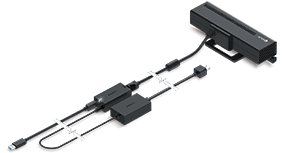
\includegraphics[width=8cm]{KinectAdapter.png}
\caption{\emph{The Kinect 2.0 camera connected to the adapter}}
\label{fig: kinect}
\end{center}
\end{figure}

The camera has to be placed horizontally in order to function correctly. The distance between the user and the camera may vary between 1.5 and 4 meters, depending on the height of the user and the size of the used screen (see figure \ref{fig: kinect_setup}). The camera can be tilted upwards or downwards. The chosen angle depends on the height of the camera. Both can be chosen freely by the user, but the user has to ensure that he is fully visible at the position he stands. The GUI allows him to verify this. A possible configuration that works well is to have to Kinect camera pointing straight ahead on a table with a height of approximately 0.8 meters.\\

\begin{figure}[H]
\begin{center}

\includegraphics[width=8cm]{KUL.png}
\caption{\emph{Setup for the Kinect camera}}
\label{fig: kinect_setup}
\end{center}
\end{figure}

Before starting the application, it is recommended to put the executable file in a directory that does not need to change of the course of multiple uses. The reason is that a subdirectory is created in the same directory, containing all data files of saved exercises. As long as this data folder and the executable are in the same directory, all previously recorded exercises are loaded when starting the application. If they get separated, the application still can be used, but it appears as if there are no saved exercises and it creates a new data folder in the directory the executable is stored.\\


\section{Graphical user interface}

%DELETE THE ITEMIZATION BELOW
\begin{itemize}
\item Procesbeschrijving, opties tussen verschillende types van interfaces (mime/music conductor)
\item Experimentele manier om tot prototype te komen door gesprek met kinesist
\item Beschrijving van de voorgestelde oplossing, beelden van de GUI, bespreking
\item Klassendiagramma voor GUI
\item \ldots
\end{itemize}

\subsection{Prototypes}

%TODO alles over de prototypes (ook experimentele strategie uitleggen)

\subsection{Description of the interface}

%TODO beschrijving + afbeeldingen van de uiteindelijke interface

\subsection{Software}

\begin{figure}[H]
\begin{center}

\includegraphics[width=8cm]{KUL.png} %PLACEHOLDER, CHANGE THE FILENAME
\caption{\emph{The class diagram of the application, focusing on the GUI}}
\label{fig: gui_classdiagram}
\end{center}
\end{figure}

%TODO klassendiagramma van de GUI + eventuele snippets uit de code (+ uitleg)


\section{Back-end software}
\label{section: Back-end software}

The focus of the application is reflected by the structure of the code. The class diagram shows a model-view pattern do make a distinction between the graphical interface of the application and the back-end (see figure \ref{fig: backend_classdiagram}).\\

\begin{figure}[H]
\begin{center}

\includegraphics[width=8cm]{KUL.png}
\caption{\emph{The class diagram of the application, focusing on the back-end}}
\label{fig: backend_classdiagram}
\end{center}
\end{figure}


The \classname{Model} class forms the core of the application. It controls the flow of the program and has collections of all important objects. An instance of \classname{Frame} can be seen as a single picture taken by the Kinect camera.

The Kinect camera has the ability to identify and measure the position relative to the camera of 25 points of a person, for instance: left elbow, right elbow, head, center of the spine, left wrist,\ldots All of these points are referred to as \classname{Joint}s and can be accessed using the libraries that come as part of the Kinect SDK installation. Each \classname{Joint} has a $x$, $y$ and $z$ coordinate, so it is unambiguously defined in space.\\

When the Kinect measures all of the \classname{Joint}s at one specific point in time, these all 25 \classname{Joint}s together form one frame. This can be seen as a single picture of a person taken by the camera. Analogous to a movie, which is a quick succession of a series of pictures, a \classname{Gesture} collects all \classname{Frame}s, which all together, contain information about how the person moved over a period of time.\\



\section{Gesture recognition}

\subsection{Support vector machine}

In order to provide enough flexibility concerning the type of exercises, SVM is used. SVM supports supervised machine learning and its use encompasses two modes: train and predict.\\

A model can be trained with a given set of data and a label to classify the gesture. The amount of numbers in one data set is referred to as the number of features. If it contains $n$ features, the entire data set can be seen as a single point in a $n$-dimensional space. It is possible to train the same gesture more than once. In that case, the same label is used to indicate that the given data set is related to the same gesture. In other words, all trainings of the same gesture are linked to the same label. All of these trained gestures with the same label are seemingly similar, but actually contain variations due to noise during the measurement of the gesture or a slightly varying execution of the gesture.\\

After training all required gestures, a SVM model is created. Given a data set of a gesture, this model can predict which of the trained gestures has the biggest resemblance to the given data set. As a result, the label of the most similar trained gesture is returned. This also explains the necessity of having multiple trainings recorded for each gesture. Errors in a single training due to noisy measurements of the Kinect camera can lead to wrong predictions. Having multiple trainings minimizes the influence noise has on the prediction and keeps into account that the user executes all gestures with slight variations. As a result, the model can predict more accurately which gesture is performed.\\

However, there are some things to keep in mind when applying this strategy. Firstly, while inputting multiple repeats of the same gesture helps with predicting the gesture after a model is created, it takes more time for the therapist to do this. Secondly, when trying to predict a gesture, the generated SVM model always returns the label of the most similar gesture, even if they are not related at all.\\

These problems are tackled as part of the approach to using SVM to predict gestures.


\subsection{Approach}

As stated in section \ref{section: Back-end software}, a gesture consists of multiple frames. Each frame contains 25 joints and each joint consists of an $x$, $y$ and $z$ component. This results in a total of 75 features that are being considered for each frame.\\

Two approaches are considered when it comes down to learning how to recognize gestures. By directly comparing these approaches, it is easier to identify their advantages and disadvantages.\\

The first approach is to add a time stamp to each frame as an extra feature, which indicates the time relative to the first frame of the gesture. This results in having 76 features per frame. If performing a certain gesture takes about $t$ seconds and is captured at a rate of $f$ frames per second, this amounts to 76 $tf$ features. This additional feature can be used to make sure that the gesture isn't just similar in space, but also in time. For a 3-second gesture recorded at 30 frames per second, which is the highest sampling speed of the Kinect camera, this amounts to 6840 features for a single training of the gesture. In other words, the number of features of one training depends on the duration of the gesture. The entire gesture is classified as a single gesture. During prediction, a gesture with the same number of features can be input to verify if that gesture matches any of the trained gestures.\\

There are several problems with this first approach. If the number of features of the gesture used for predicting does not match the number of features of the training gestures, the prediction is not accurate and should be discarded. Discarding is necessary as SVM always returns the label of a gesture, even if the predicted gesture is completely unrelated to any of the trained gestures. This poses a problem as different gestures can have a different duration. Even different trainings of the same gesture can take for instance 3 seconds and 3.1 seconds, implying that the recordings have a different number of frames and thus a different number of features. A possible solution is to recalculate the entire gesture and use interpolation to convert the set of frames to a new set with a known, fixed size and preferably with equidistant time stamps.\\

Furthermore, not just the trainings of one gesture, but all of the gestures need to have the same number of frames. The gesture to predict is not known beforehand and can only be predicted accurately if the number of features for both the predicted gesture and trained gesture are equal. As a result, it is required that all gestures have an equal amount of features. This means that short gestures need to be mathematically extended with additional frames to match the size of longer gestures. Another side effect is that all gestures need to have the same duration, not just the same amount of features. This limits the therapist in choosing exactly what exercises he wants the patient to perform. Also, predicting a gesture can only be as fast as the trained gesture with the longest duration. More in particular, assume the longest gesture is 5 seconds in length. It then follows that it takes about 5 seconds to predict any gesture. This also means that patients that control the game can only perform one action every 5 seconds. As the games to be played are unknown beforehand, a slow reaction time of the application can render some games unplayable. As such, this approach is not viable.\\

The second approach is to split up one gesture into $n$ smaller gestures and classify each of them differently, assigning a different label to each part of the gesture. Assume that a gesture is split up into 4 smaller parts so that each part contains approximately an equal amount of frames. Consider a 4-second gesture sampled at 30 frames per second. The complete gesture consists of 120 frames. By splitting it up into 4 parts, each part contains 30 frames. All first 30 frames are labeled with the same label, for instance 1. The next 30 frames receive a label 2, and so on. To put it differently, the considered gesture is split up into 4 postures with each having 30 slightly varying trainings. In contrast to the first approach, as described above, prediction does not happen for an entire gesture, but for separate postures. The condition for having executed the entire gesture is that each of the postures are predicted correctly and in the right order. To put it differently, $n$ \emph{pictures} are taken of the gesture and if at some point during prediction all pictures are executed in the right order, the application acknowledges the execution of the gesture.\\

AFBEELDING NODIG MET EXTRA UITLEG IN ALINEA HIERBOVEN\\

The biggest advantage of this approach is the flexibility of it. Each posture corresponds to a single frame, which contains 75 features. This eliminates the need of having gestures with the same length or having to modify training data to have gestures with an equal number of features. It is even possible to not just link a gesture, but also a posture to a keyboard button, which allows the physical therapist to choose the exercises that fit the needs of a patient the best. Additionally, the application reacts immediately to an executed gesture, not after a fixed amount of time. This allows for a wider variety of games being playable using this application.\\

Another advantage is that it solves the issue where SVM always returns the label of a predicted gesture, even when the patient is not doing anything. A gesture is only recognized when all parts of it are executed. In other words, gestures are not recognized involuntarily and, as such, actions like button presses that influence the game are not executed by accident. This also means that no neutral or \emph{wrong} gestures are required to link a certain gesture to no in-game action.\\ %TODO verduidelijken

The disadvantage of this second approach is that there is no strict requirement for the entire gesture to be executed in about the same time as the gesture recorded during training. If a gesture is executed faster during prediction compared to during training, it is recognized as the same gesture being executed. However, it is possible to solve this timing issue to some extent when the gesture during predicting is performed slower. The gesture can be ignored if more than a certain amount of time passes. This time threshold takes the gesture with the longest duration into account and is chosen higher than this in order to allow all gestures to be executed and successfully recognized.